\section{Objects in the amber.crawler package}



\classname{RSS}

\begin{classmetadata}
  \extends{CrawlerObject}
  \implements{AirBrushCallable}
  \processing{An RSS object will accept messages to set its feed source, i.e.
      the feed it should crawl. A message of type `Feed.RSS' or `Feed.Atom'
      will set the source to that URL, whereas a message of type `Feed.OMPL'
      will result RSS to parse this and set all URLs in the \ac{OPML} document
      as source URL.

      It will only post messages of the type `Story' as they are described in
      Section~\ref{sct:messages:story}. No other messages are sent.}
\end{classmetadata}

\begin{interface}
  \init{RSS}{}
    {Creates a new RSS crawler. It will wait for instructions via Psyclone,
      like which RSS feed has to be monitored.}
  \init{RSS}{URL feedurl}
    {Creates a new RSS crawler, initialized with the URL of the feed to be
      monitored.}
  \method{void}{airBrushReceiveMessage}{Message msg}
    {Callback function for AirBrushCallable. It will handle incoming messages
        of the type `Feed.RSS', `Feed.Atom' and `Feed.OPML'. With the OPML type
        it is possible to let a crawler handle more than one feed.}
  \method{void}{run}{}
    {Callback function for Runnable.}
\end{interface}

\begin{figure}
  \centering
  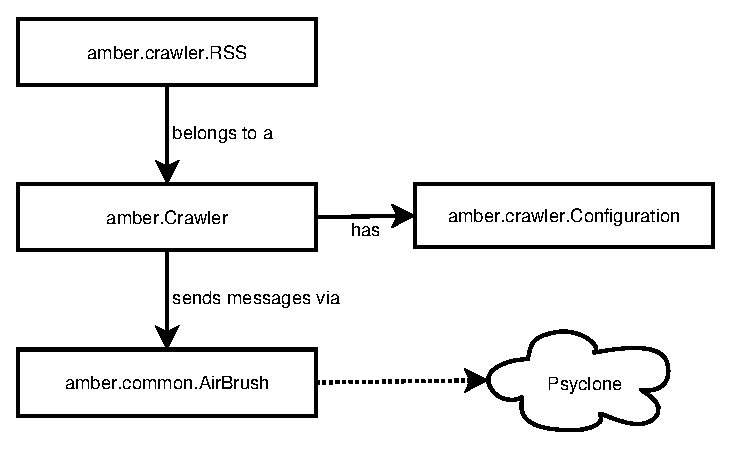
\includegraphics{image/crawler}
  \caption{
    Diagram of the design of the Crawler, the names are Java classnames, arrows
    mean that calls exist in the direction of the arrow.
  }
\end{figure}

